% Chapter Template

\chapter{Introduction} % Main chapter title

\label{Chapter1} % Change X to a consecutive number; for referencing this chapter elsewhere, use \ref{ChapterX}

As humanity strives to better understand the world and universe around it, the physical limitations of our species become more and more apparent. While we have made considerable progress in our struggles to move forward, such as being able to record the movement of a light particle on camera despite it being the fastest moving object we know of so far\textsuperscript{\cite{velten2013femto}}, or being able to capture an image of a black hole\textsuperscript{\cite{landau_2019}}, such achievements would not have been possible if our scientists did not have realistic expectations of how they should approach these challenges, or the expected results. 

In order to achieve what they have, scientists needed to first understand the phenomena they were studying: the light having the particular properties of both particle and wave and the ability of black holes to distort space around them. All of this would not have been possible without simulations. 

%----------------------------------------------------------------------------------------
%	SECTION 1
%----------------------------------------------------------------------------------------

\section{Electromagnetic Simulations}
With the fast development of technology came new opportunities for gaining a better understanding of vast natural phenomena. We will be focusing on one of them, that being Electromagnetic Wave Propagation. 

As one can imagine, analyzing electromagnetic fields through plain observation is near impossible, with only a few exceptions\textsuperscript{\cite{cao2005first}}. Even if we supposed that it was possible to easily achieve an acceptable amount of information from observing experiments, the cost and quality of the resulting data would mostly be of scientific use, with little to no practical use whatsoever. Considering that electromagnetic waves are widely used in almost every industry, either as part of the building process or as a finished product, having data that cannot be used practically does not help. 

That is why, thanks to the progress made in the computational capabilities of computers so far and the use of the theories and formulas gathered from past scientific endeavors, one can create data that is a close approximate of reality. Both shall be discussed in this chapter, but we cannot proceed without first going into what is believed by scientists to be the equations that govern large-scale electromagnetic phenomena\textsuperscript{\cite{stratton2007electromagnetic}}: Maxwell Equations.

%-----------------------------------
%	SUBSECTION 1
%-----------------------------------
\subsection{Maxwell Equations}

As mentioned above, Maxwell Equations are believed to dictate the behavior of all kinds of electromagnetic fields at a macroscopic level. These equations are the following:

\begin{equation}
	\label{eqn:electricinduction}
	\vec{\nabla} \times \vec{E}(\vec{r},t) = - \frac{\partial \vec{B}(\vec{r},t)}{\partial t}
\end{equation}
\begin{equation}
	\label{eqn:amperesLaw}
	\vec{\nabla} \times \vec{H}(\vec{r},t) = \vec{J}(\vec{r},t) + \frac{\partial \vec{D}(\vec{r},t)}{\partial t}
\end{equation}
\begin{equation}
	\label{eqn:magneticDivergence}
	\vec{\nabla} \cdot \vec{B}(\vec{r},t) = 0
\end{equation}
\begin{equation}
	\label{eqn:gausslaw}
	\vec{\nabla} \cdot \vec{D}(\vec{r},t) = \rho (\vec{r})
\end{equation}

To give a brief explanation over the meaning of each equation:

Equation \ref{eqn:electricinduction} explains the effects of the electric field $\vec{E}$ on the rate of change of the magnetic induction $\vec{B}$. This can also be referred to as the equation of electromagnetic induction, where the right hand side is the EMF or voltage and the left hand side is the magnetic flux. To those who study this particular area of physics, this equation will seem familiar, because it was derived from Faraday's law of induction.

\begin{figure}
	\centering
	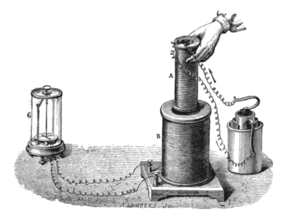
\includegraphics{Figures/faradayexp}
	\decoRule
	\caption[Faraday's Experiment]{Faraday's Experiment,\textsuperscript{\cite{poyser1918magnetism}}} which resulted in the law that was later used by Maxwell in making his equation.
	\label{fig:faradayexp}
\end{figure}

Equation \ref{eqn:amperesLaw} is also known as Ampère–Maxwell law, because although it originated from Ampère, the current form was derived by Maxwell to include the magnetic current density $\vec{J}$. The equation explains the effects of the magnetic field on the electric current.

Equation \ref{eqn:magneticDivergence}, otherwise known as Gauss's law for magnetism, talks about the divergence of the magnetic field. According to this law the divergence is always 0. What this means is that in a magnetic field there is no such thing as a source (positive divergence) or a sink (negative divergence), rather a magnetic field can be more closely compared to a closed loop that flows in one direction. That is why every magnet that we know of has two poles. To translate this into something more easily understandable, it basically means that, if we were to pick any subset of the area of a magnetic field, no matter what area we pick, we would have vector fields going inside this area, and vector fields going outside in equal number. A simple representation of this rule can be seen in \ref{fig:magneticdivergence}, where it can be noted that the number of vectors heading towards the north pole are equal to the vectors going outside of it. Interestingly enough, if the bar magnet were to be cut in half, then the result would be two smaller bar magnets with 2 poles each and the exact same vector field.

\begin{figure}
	\centering
	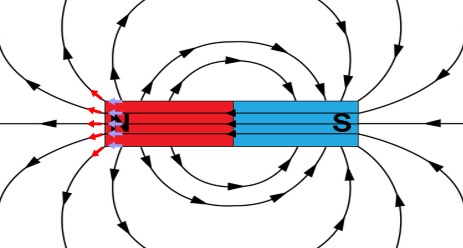
\includegraphics[scale=0.9]{Figures/magneticdivergence}
	\decoRule
	\caption[Magnetic Divergence]{A crude representation of magnetic divergence through the use of a bar magnet.}
	\label{fig:magneticdivergence}
\end{figure}

Equation \ref{eqn:gausslaw}, is the main Gauss law for electric currents. It looks rather similar to his law of magnetism on the left hand side; the previous magnetic divergence is now replaced with the electric divergence. The bigger difference is the $\rho$ on the right hand side, which is the density of charge of the electric field. In basic terms, it means that the divergence of the electric field is equal to the charge density for that point.

For the above equations, we also have the following material relations which will be useful later on:
\begin{equation}
	 \vec{D}(\vec{r},t) = \epsilon(\vec{r}) \cdot \vec{E}(\vec{r},t)
\end{equation}
\begin{equation}
	\vec{B}(\vec{r},t) = \mu(\vec{r}) \cdot \vec{H}(\vec{r},t)
\end{equation}

The equations above are shown in their derivative form, but they can also be shown as their integral equivalent. There is no difference in implementation, regardless of which form is used.

%-----------------------------------
%	SUBSECTION 2
%-----------------------------------

\subsection{Solving the Wave Equation}
Morbi rutrum odio eget arcu adipiscing sodales. Aenean et purus a est pulvinar pellentesque. Cras in elit neque, quis varius elit. Phasellus fringilla, nibh eu tempus venenatis, dolor elit posuere quam, quis adipiscing urna leo nec orci. Sed nec nulla auctor odio aliquet consequat. Ut nec nulla in ante ullamcorper aliquam at sed dolor. Phasellus fermentum magna in augue gravida cursus. Cras sed pretium lorem. Pellentesque eget ornare odio. Proin accumsan, massa viverra cursus pharetra, ipsum nisi lobortis velit, a malesuada dolor lorem eu neque.

%----------------------------------------------------------------------------------------
%	SECTION 2
%----------------------------------------------------------------------------------------

\section{Finite Difference Time Domain Method}

Sed ullamcorper quam eu nisl interdum at interdum enim egestas. Aliquam placerat justo sed lectus lobortis ut porta nisl porttitor. Vestibulum mi dolor, lacinia molestie gravida at, tempus vitae ligula. Donec eget quam sapien, in viverra eros. Donec pellentesque justo a massa fringilla non vestibulum metus vestibulum. Vestibulum in orci quis felis tempor lacinia. Vivamus ornare ultrices facilisis. Ut hendrerit volutpat vulputate. Morbi condimentum venenatis augue, id porta ipsum vulputate in. Curabitur luctus tempus justo. Vestibulum risus lectus, adipiscing nec condimentum quis, condimentum nec nisl. Aliquam dictum sagittis velit sed iaculis. Morbi tristique augue sit amet nulla pulvinar id facilisis ligula mollis. Nam elit libero, tincidunt ut aliquam at, molestie in quam. Aenean rhoncus vehicula hendrerit.

\section{FDTD Implementation}

Sed ullamcorper quam eu nisl interdum at interdum enim egestas. Aliquam placerat justo sed lectus lobortis ut porta nisl porttitor. Vestibulum mi dolor, lacinia molestie gravida at, tempus vitae ligula. Donec eget quam sapien, in viverra eros. Donec pellentesque justo a massa fringilla non vestibulum metus vestibulum. Vestibulum in orci quis felis tempor lacinia. Vivamus ornare ultrices facilisis. Ut hendrerit volutpat vulputate. Morbi condimentum venenatis augue, id porta ipsum vulputate in. Curabitur luctus tempus justo. Vestibulum risus lectus, adipiscing nec condimentum quis, condimentum nec nisl. Aliquam dictum sagittis velit sed iaculis. Morbi tristique augue sit amet nulla pulvinar id facilisis ligula mollis. Nam elit libero, tincidunt ut aliquam at, molestie in quam. Aenean rhoncus vehicula hendrerit.

\subsection{Project Plan, Requirements, and Tools Used}

Sed ullamcorper quam eu nisl interdum at interdum enim egestas. Aliquam placerat justo sed lectus lobortis ut porta nisl porttitor. Vestibulum mi dolor, lacinia molestie gravida at, tempus vitae ligula. Donec eget quam sapien, in viverra eros. Donec pellentesque justo a massa fringilla non vestibulum metus vestibulum. Vestibulum in orci quis felis tempor lacinia. Vivamus ornare ultrices facilisis. Ut hendrerit volutpat vulputate. Morbi condimentum venenatis augue, id porta ipsum vulputate in. Curabitur luctus tempus justo. Vestibulum risus lectus, adipiscing nec condimentum quis, condimentum nec nisl. Aliquam dictum sagittis velit sed iaculis. Morbi tristique augue sit amet nulla pulvinar id facilisis ligula mollis. Nam elit libero, tincidunt ut aliquam at, molestie in quam. Aenean rhoncus vehicula hendrerit.


\subsection{Computational Limitations and Inaccuracies Explained}

Sed ullamcorper quam eu nisl interdum at interdum enim egestas. Aliquam placerat justo sed lectus lobortis ut porta nisl porttitor. Vestibulum mi dolor, lacinia molestie gravida at, tempus vitae ligula. Donec eget quam sapien, in viverra eros. Donec pellentesque justo a massa fringilla non vestibulum metus vestibulum. Vestibulum in orci quis felis tempor lacinia. Vivamus ornare ultrices facilisis. Ut hendrerit volutpat vulputate. Morbi condimentum venenatis augue, id porta ipsum vulputate in. Curabitur luctus tempus justo. Vestibulum risus lectus, adipiscing nec condimentum quis, condimentum nec nisl. Aliquam dictum sagittis velit sed iaculis. Morbi tristique augue sit amet nulla pulvinar id facilisis ligula mollis. Nam elit libero, tincidunt ut aliquam at, molestie in quam. Aenean rhoncus vehicula hendrerit.